\documentclass[a4paper]{kulakarticle}

\usepackage[utf8]{inputenc}
\usepackage[dutch]{babel}
\usepackage{titling}
\title{Kost van een Airbnb-verblijf}
\author{Project statistiek}
\date{Academiejaar 2022 -- 2023}
\address{
	Louis Vandenbruwaene\\
	Jasper Denorme\\
	Dieter Demunck}
\usepackage{graphicx,flafter,framed,caption}
\usepackage{amsfonts,amssymb,amsmath,textcomp,eurosym,wasysym}
\usepackage{listings}
\usepackage{siunitx}
\sisetup{output-decimal-marker={,}}
\usepackage{enumitem}
\usepackage{multicol}
\usepackage{caption}
\usepackage{tabularx,array}
\newcommand{\rood}[1]{\textcolor{red}{#1}}

\begin{document}
	\maketitle
	\section*{Inleiding}
	Airbnb is een online platform (\href{https://www.airbnb.com}{\texttt{www.airbnb.com}}) waarop reizigers een kort verblijf kunnen boeken in een accommodatie (bv. een kamer, een huis, een woonboot, …) die door particulieren wordt verhuurd. Airbnb werd opgericht in 2008 en is ondertussen een erg populair alternatief geworden voor de traditionele hotels. \\
	
	Dit onderzoek focust op de totale kostprijs voor het huren van een Airbnb-verblijf in Amsterdam voor twee personen gedurende een weekend (vrijdag tot zondag). Er wordt nagegaan met welke factoren deze kostprijs samenhangt en in welke mate de kost daarmee kan worden voorspeld. Hierbij wordt er gebruik gemaakt van een aantal veranderlijken verzameld in het kader van een onderzoeksproject uitgevoerd door Kristóf Gyódi en Łukasz Nawaro. Het gaat enerzijds over kenmerken van het verblijf en tevredenheid van eerdere gasten volgens de gegevens van Airbnb, anderzijds over de ligging van het verblijf ten opzichte van het stadscentrum, bezienswaardigheden en restaurants, telkens rekening houdend met de populariteit, zoals gerapporteerd door TripAdvisor.\\
	
	Tabel \ref{beschrijving} beschrijft de variabelen en tabel \ref{uitreksel} geeft enkele basisstatistieken weer van de veranderlijken die gebruikt worden in het onderzoek. \\\\

\begin{table}[h]
	\centering
	\begin{tabular}{c|p{10cm}}
		\raggedright
		Naam & Beschrijving\\
		\hline
		realSum & Som van alle kosten in euro\\ 
		room & Soort verblijf (1 = volledige woning, 2 = afzonderlijke kamer, 
		3 = gedeelde kamer) \\ 
		capacity & Maximaal aantal gasten \\
		bedrooms & Aantal beschikbare slaapkamers in het verblijf \\
		dist & Afstand tot het stadscentrum (km) \\
		metro & Afstand tot dichtstbijzijnde metro-halte (km)\\
		attr & Attractiescore, nabijheid van bezienswaardigheden \\
		rest & Restaurantscore, nabijheid van restaurants \\ 
		host & Type verhuurder (0 = enige beschikbare woning, 1 = 2 tot 4 beschikbare woningen,
		2 = meer dan 4 beschikbare woningen) \\ 
		cleanliness & Modale score voor netheid van het verblijf volgens gasten (op 10) \\
		satisfaction & Tevredenheid van de gasten (op 10)\\
		
	\end{tabular}
	\caption{Beschrijving van de gebruikte veranderlijken.}
	\label{beschrijving}
\end{table}
\begin{table}[h]
	\centering
	\begin{tabular}{| l| l| l|  p{5cm} |}
		\hline
		Naam & Gemiddelde $\pm$ standaardfout  & Bereik & Algemene vorm\\  [1ex]
		\hline\hline
		realSum & $604.8\pm 443.6828 $ & $7964.755$  &  zeer rechtsscheef\\    [0.5ex]
		\hline
		capacity & $2.77\pm 1.019876$ & $4$  & rechtsscheef \\[0.5ex]
		\hline
		bedrooms & $1.303\pm 0.7329492$ & $5$ & rechtsscheef \\[0.5ex]
		\hline
		dist & $2.80634\pm 2.036602$  & $11.18089$ & zeer rechtsscheef \\  [0.5ex]
		\hline
		metro & $1.0892\pm 0.8265551$ & $4.375388$ & zeer rechtsscheef \\ [0.5ex]
		\hline
		attr & $2.101\pm 0.9407762$ & $9$  & rechtsscheef \\  [0.5ex]
		\hline
		rest & $3.285\pm 1.760009$ & $9$ & benaderend lognormaal met zware staarten \\ [0.5ex]
		\hline
		cleanliness & $9.471\pm 0.8306492$ & $8$ & benaderend exponentieel  \\ [0.5ex]
		\hline
	\end{tabular}
	\caption{Basisstatistieken van de gebruikte veranderlijken.}
	\label{uitreksel}
\end{table}
	
	\section{Methode}
	\rood{Deze sectie telt hoogstens één pagina (exclusief figuren en tabellen).}
	\subsection{Kenmerken van de steekproef}
Om te testen of de gemiddelde kost veranderd is tegenover 2019, maken we gebruik van een student t-test voor één gemiddelde. We mogen deze gebruiken, want de dataset voldoet aan de centrale limietstelling (n = 977). Om na te gaan of het aandeel particuliere verhuurders groter is dan het aantal professionele verhuurders, hebben we van een $z$-test voor één proportie gebruikt.\\
 
 We zijn via een $\chi ^2$-test nagegaan of het aantal beschikbare kamers Poisson verdeeld is. Dit deden we nadat we data bij elkaar hebben gegooid, om aan de Cochranregel te voldoen.
	
	\subsection{Gemiddelde kost}
	
	Hier zal onderzocht worden of de totale prijs van een verblijf voor twee personen afhankelijk is van bepaalde andere variabelen.
	De eerste hypothese is dat de totale prijs afhankelijk is van het al dan niet behalen van de maximale netheidsscore. We testen hierbij het verschil tussen verblijven met en zonder de maximumscore voor netheid.
	De tweede hypothese is dat deze prijs verschilt naargelang de eigenaar slechts één verblijf aanbiedt, of meerdere.
	De laatste hypothese is dat de prijs verschilt naargelang de volledige woning wordt verhuurd, of enkel een deel ervan.
	Aangezien de variantie nooit gekend is, werd bij alle drie de hypotheses eerst de normaliteit van de twee categorieën getest aan de hand van de Shapiro-Wilk-test. Hierna wordt een t-test voor twee gemiddelden bij verschillende varianties uitgevoerd. Deze laatste test mag uitgevoerd worden, omdat de centrale limietstelling (CLS) voldaan is, alhoewel de steekproefwaarden blijken af te wijken van normaliteit.

	\subsection{Associatie met de verschillende veranderlijken}
	

	Verder wordt de associatie tussen \textbf{realsum} en de andere veranderlijken onderzocht. Aangezien \textbf{realsum} niet normaal verdeeld is (zie figuur \ref{fig:clean1}) en er zelden samenvallende waarden voorkomen, wordt getest of de Spearman rangcorrelatie van de prijs met de continue variabelen significant van nul verschilt. Om de afhankelijkheid met de discrete en kwalitatieve variabelen te bepalen, wordt een $\chi ^2$-test gebruikt. Hiervoor wordt gewerkt met de gediscretiseerde \textbf{realsum}. Ook de discrete en kwalitatieve variabele worden samengevoegd om zo goed mogelijk aan de Cochranregel te voldoen. Enkel \textbf{host} blijft onveranderd. \textbf{Realsum} wordt verdeeld volgens zijn $4$ kwantielen en de andere opdelingen zijn te vinden in tabel \ref{grenzen}\\\\
	\begin{table}[h]
		\centering
			\begin{tabular}{c|c}
			\centering
			naam& opdelende grenzen\\
			\hline
			\textbf{cleanliness} & $ 0 $ - $ 7.5 $ - $ 8.5$ - $ 9.5 $ - $ 10.5$ \\
			\textbf{capacity}& $-0.5$ - $2.5$ - $3.5$ - $4.5$ - $6.5$\\
			\textbf{bedrooms}& $-0.5$ - $0.5$ - $1.5$ - $2.5$ - $6$\\
			\textbf{room} & $0.5$ - $1.5$ - $3.5$\\
			\end{tabular}
			\caption{De grenzen, die de gegevens opdelen zodat de aan Cochran-regel voldaan is.}
			\label{grenzen}
	\end{table}
	\subsection{Verklaren van de kost}
	
	We zullen hier trachten \textit{realSum} te verklaren aan de hand van de andere veranderlijken. Dit gebeurt met een lineair regressiemodel. Eerst wordt het model gemaakt enkel op basis van
	de variabele \textit{attr}. Er wordt ook bestudeerd of een model gebaseerd op de $log_{10}$-transformatie van deze veranderlijke, $log_{10}$(\textit{attr}), een beter resultaat geeft, aangezien deze variabele rechtsscheef verdeeld is: skewness = 2,454883.
	Daarna wordt er via achterwaartse regressie een meervoudig regressiemodel gezocht, waar we alle continue variabelen voor gebruiken. Ten slotte wordt nog bestudeerd of de binaire variabele \textit{dummy}, \textit{room} == volledige woning, een
	significante invloed heeft op het model.
	
	
	\section{Resultaten}
	\rood{Deze sectie telt hoogstens één pagina (exclusief figuren en tabellen).}
	\subsection{Kenmerken van de steekproef}
De gemiddelde kost in de steekproef is 604 euro, terwijl deze in 2019 620 euro was. Het verschil van 16 euro is niet significant ($t_{976}$ = -1.1, p = 0.29). We kwamen uit dat $p \approx 0$ voor onze test op het aandeel van particuliere vs. professionele verhuurders. We bekomen een verschil van 295. Bij de $\chi$-kwadraat test voor onze verdeling bekomen we $\chi^2 = 424.77$ en $p \approx 0$, we kunnen dus aannemen dat het aantal beschikbare kamers niet Poisson verdeeld is.
	
	\subsection{Gemiddelde kost}
	
	We merken uit de gegevens in tabel \ref{tab:intermediary_results_gemiddelde_kost} dat elke categorie minstens 200 datapunten bevat, waardoor we kunnen veronderstellen dat de centrale limietstelling (CLS) geldig is. Uit de resultaten van de Shapiro-Wilk-testen volgt ook dat we met aan zekerheid grenzende waarschijnlijkheid kunnen veronderstellen dat geen enkele categorie normaal verdeeld is.
	
	Uit de resultaten van de t-testen bij verschillende varianties in tabel \ref{tab:end_results_gemiddelde_kost} merken we dat er op basis van de steekproef met aan zekerheid grenzende waarschijnlijkheid een verschil bestaat tussen de gemiddelde kost voor een verblijf van twee personen bij verblijven waarbij de volledige woning wordt verhuurd ten opzichte van verblijven waar maar een deel wordt verhuurd, waarbij volledige woningen gemiddeld €185 duurder zijn. We merken ook dat er een redelijke aanwijzing is dat het aantal verblijven dat een gastheer verhuurt een verschil zou betekenen in prijs. Hierbij zijn verblijven bij gastheren met meerdere woningen gemiddeld ongeveer €52 goedkoper.
	
	Over het verschil in prijs voor twee personen voor verblijven met of zonder de maximum netheidsscore valt weinig te concluderen, aangezien de p-waarde net onder de verwerpingsgrens ligt. Dit zou toeval kunnen zijn, maar zou ook een aanwijzing kunnen zijn voor een werkelijk verschil in prijs, waarbij verblijven onder de maximum netheidsscore gemiddeld ongeveer €35 goedkoper zouden zijn.
	
	\begin{table}
		\caption{Aantal datapunten, gemiddelde, en p-waarde van de Shapiro-Wilk-test (uitgevoerd op deze datapunten) van de kost voor een verblijf van 2 personen, gefilterd op bepaalde gegevens.}
		\label{tab:intermediary_results_gemiddelde_kost}
		\begin{tabular}{|l*{3}{|r}|}
			\hline
			Kost voor 2 personen bij ...        & Aantal & Gemiddelde & Shapiro-Wilk-test p-waarde \\ \hline
			\hline
			Maximumscore netheid                & 376    & $457.1111$ & $< 2.2 \cdot 10^{-16}$ \\ \hline
			Niet maximumscore netheid           & 215    & $422.2669$ & $3.091 \cdot 10^{-12}$ \\ \hline
			Gastheer verhuurt 1 woning          & 367    & $463.9553$ & $< 2.2 \cdot 10^{-16}$ \\ \hline
			Gastheer verhuurt meerdere woningen & 224    & $412.4534$ & $< 2.2 \cdot 10^{-16}$ \\ \hline
			Volledige woning wordt verhuurd     & 288    & $539.0370$ & $< 2.2 \cdot 10^{-16}$ \\ \hline
			Deel van de woning wordt verhuurd   & 303    & $354.5165$ & $< 2.2 \cdot 10^{-16}$ \\ \hline
		\end{tabular}
	\end{table}

	\begin{table}
		\caption{Verschil in gemiddelden, en p-waarde van de t-testen (bij verschillende varianties) op het verschil tussen twee categorieën van de kost van een verblijf voor twee personen.}
		\label{tab:end_results_gemiddelde_kost}
		\begin{tabular}{|l*{2}{|r}|}
			\hline
			Verschil in kost voor 2 personen tussen ...  & Verschil van gemiddelden
			& t-test p-waarde \\ \hline
			\hline
			
			Maximumscore netheid of niet                 & $34.84423$
			& $0.03848$              \\ \hline
			Gastheer verhuurt 1 woning of meerdere       & $51.50189$
			& $0.002512$             \\ \hline
			Gastheer verhuurt volledige woning of deel   & $184.5205$
			& $< 2.2 \cdot 10^{-16}$ \\ \hline
		\end{tabular}
	\end{table}
	
	\subsection{Associatie met de verschillende veranderlijken}
	
	Uit tabel \ref{continue variabelen afhankelijkheid} kunnen we met aan zekerheid grenzende waarschijnlijkheid concluderen dat \textbf{realsum} afhankelijk is van elke continue variabele in de dataset. De bijhorende correlatie wordt geschat door rho.
	\begin{table}
		\begin{tabular}{c|c|c|c }
			naam & p-waarde & afhankelijkheid & rho\\
			\hline
			\hline
			dist & $< 2.2 \cdot 10^{-16} $&ja& $-0.4107378$ \\
			metro &$ 9.476\cdot 10^{-10}$& ja& $-0.1941159$ \\ 
			attr &$ < 2.2\cdot 10^{-16}$& ja&$0.4314979 $ \\
			rest &$ < 2.2\cdot 10^{-16}$& ja&$0.4276987 $ \\
			satisfaction &$ 1.657\cdot 10^{-7}$& ja&$0.1664983 $ \\
		\end{tabular}
		\caption{Afhankelijkheid van de prijs met de continue variabelen.}
		\label{continue variabelen afhankelijkheid}
	\end{table}
	Uit tabel \ref{discrete variabelen afhankelijkheid} kunnen we met aan zekerheid grenzende waarschijnlijkheid besluiten dat \textbf{realsum} afhankelijk is van: \textbf{capacity}, \textbf{bedrooms}, \textbf{room} en \textbf{host}. We kunnen ook met grote waarschijnlijkheid zeggen dat \textbf{cleanliness} niet gecorreleerd is met \textbf{realsum}. 
	\begin{table}[h]
		\begin{tabular}{c|c|c|c }
			naam & p-waarde & afhankelijkheid & $\chi ^2$\\
			\hline
			\hline
			cleanliness & $0.7775$&nee& $5.6174$ \\
			capacity &$ < 2.2\cdot 10^{-16}$& ja& $390.3$ \\ 
			bedrooms &$ < 2.2\cdot 10^{-16}$& ja&$368.1 $ \\
			room &$ < 2.2\cdot 10^{-16}$& ja&$ 337.29$ \\
			host &$ 5.506\cdot 10^{-7}$& ja&$39.581 $ \\
		\end{tabular}
		\caption{Afhankelijkheid van de prijs met de discrete en kwalitatieve variabelen.}
		\label{discrete variabelen afhankelijkheid}
	\end{table}
	
	\subsection{Verklaren van de kost}
	
	
	\section{Discussie}
	\rood{Deze sectie telt hoogstens één pagina (exclusief figuren en tabellen).}
	\subsection{Kenmerken van de steekproef}
Op basis van de steekproef lijkt er geen verandering te zijn in de kostprijs van een kamer. Met aan zekerheid grenzende waarschijnlijkheid kunnen we aannemen dat er meer particulier verhuurders zijn, het lijkt er dus op dat er een 'strenge' regulering is in Amsterdam. We kunnen ook met zeer grote waarschijnlijkheid aannemen dat het aantal beschikbare kamers niet Poisson verdeeld is.
	
	\subsection{Gemiddelde kost}
	
	% I feel like this is maybe too much....
	Uit de gegevens merken we dat de prijs van een verblijf voor twee personen praktisch zeker duurder wordt wanneer de volledige woning wordt verhuurd, wat op zich intuïtief is.
	Er is ook een duidelijke aanwijzing dat verblijven met een gastheer die meerdere woningen verhuurd goedkoper zou zijn. Een mogelijke verklaring is dat deze gastheren voorraden aankopen voor meerdere verblijven, en dus mogelijks goedkoper grotere aantallen voorraden kunnen aankopen en deze dan kunnen verdelen onder hun verblijven. Een andere verklaring is dat zij mogelijks meer competitief zijn in hun prijs, aangezien dit hun hoofdinkomen zou zijn. In tegenstelling tot een gastheer die een verblijf verhuurt als bijzaak, moeten gastheren die dit professioneel doen een zekerheid hebben op huurders.
	Er is een grote onzekerheid of er een werkelijk verschil is in prijs tussen verblijven met en zonder de maximumscore voor netheid. Een mogelijke verklaring is dat gastheren zonder de maximumscore zelf niet goed inzien hoe vuil hun verblijf is in vergelijking met propere verblijven. Aangezien vele verblijven een netheidsscore tussen 8 en 10 hebben (zie figuur \ref{fig:cleanliness}), worden meeste gasten hier misschien weinig door afgeschrokken. Een verschil zou dan te verklaren kunnen zijn doordat vuile verblijven hun prijs moeten verlagen om een redelijk aantal gasten te kunnen hebben.
	
	\begin{figure}
		\centering
		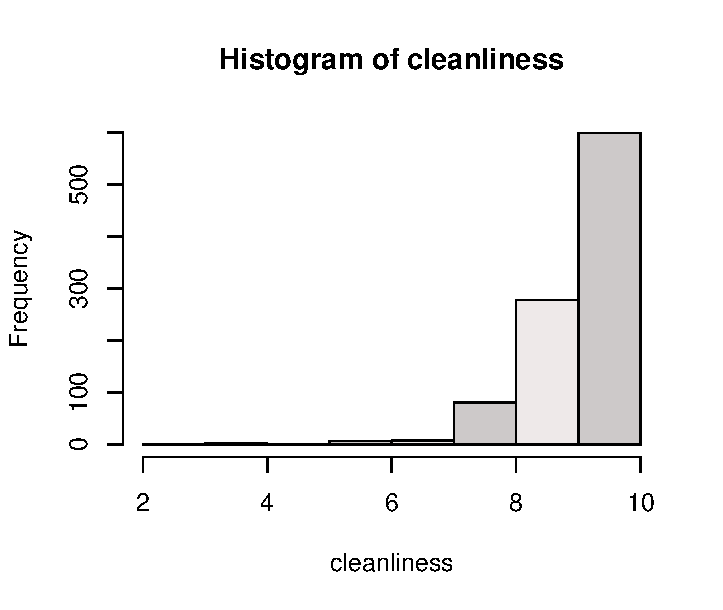
\includegraphics{Figuren/cleanliness_hist.pdf}
		\caption{Histogram van de netheidsscore}
		\label{fig:cleanliness}
	\end{figure}
	
	\subsection{Associatie met de verschillende veranderlijken}
	
	Op basis van de steekproef zijn \textbf{attr}, \textbf{rest}, \textbf{capacity}, \textbf{room}, \textbf{host}, \textbf{bedrooms} en \textbf{satisfaction} positief gecorreleerd met \textbf{realsum}. Bij de continue variabelen kunnen we dit afleiden uit de rho en bij de andere kunnen enkel kijken naar de scatterplots. Daarentegen zijn \textbf{dist} en \textbf{metro} negatief gecorreleerd met de totale prijs. Dit is duidelijk uit de waarde van rho. Intuïtief is dit ook aanvaardbaar. Toegankelijkheid tot het stadscentrum en een metrohalte verhoogt de waarde van een verblijf.
	
\begin{figure}
	\centering
	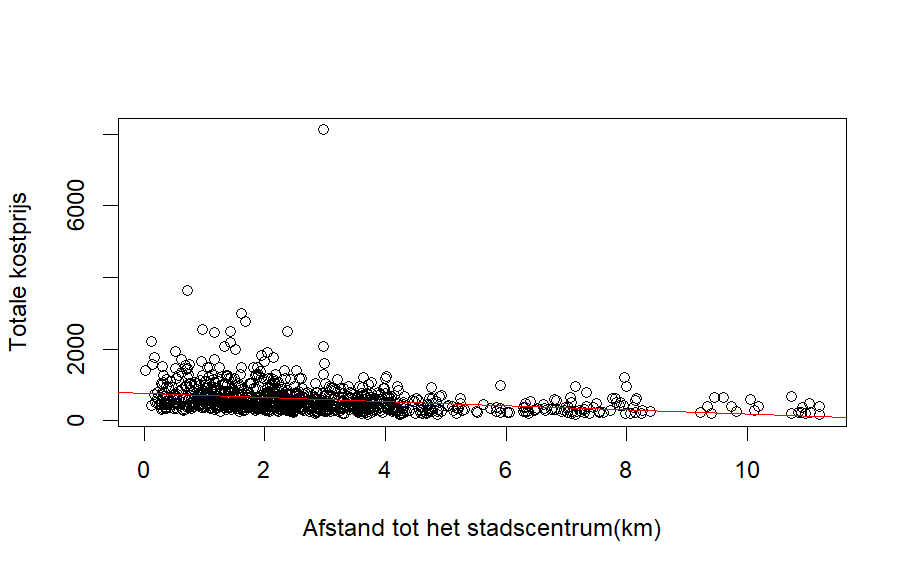
\includegraphics[width=0.49\linewidth]{Figuren/dist}
	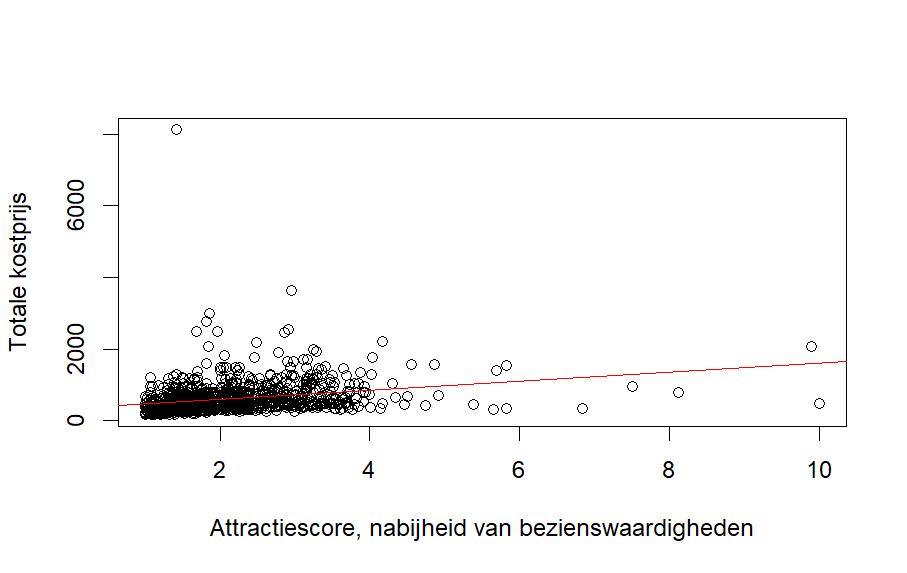
\includegraphics[width=0.49\linewidth]{Figuren/attr}
	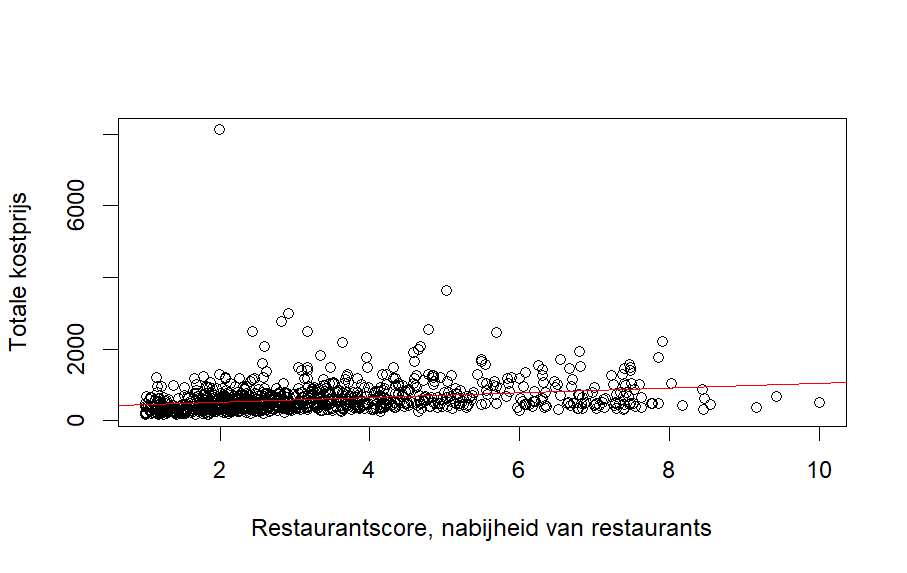
\includegraphics[width=0.49\linewidth]{Figuren/rest}
	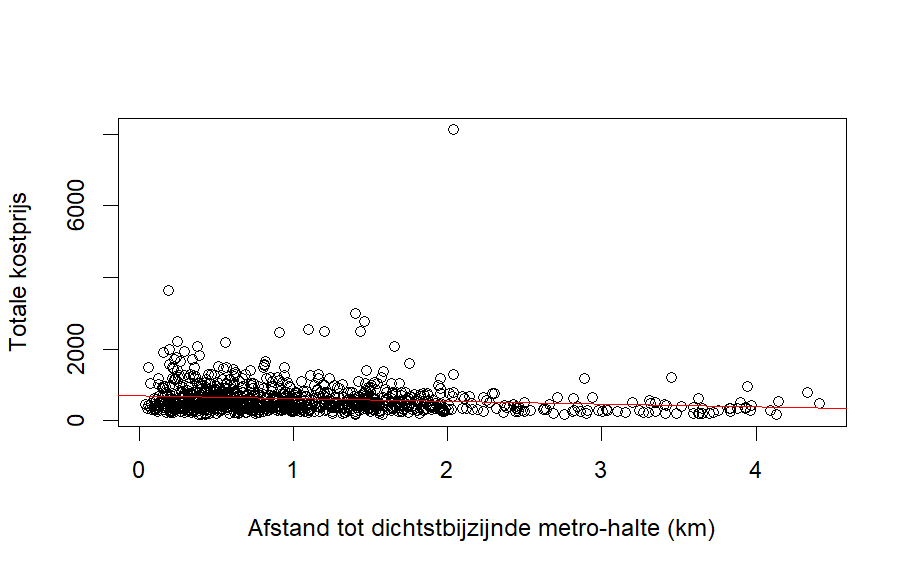
\includegraphics[width=0.49\linewidth]{Figuren/metro}
	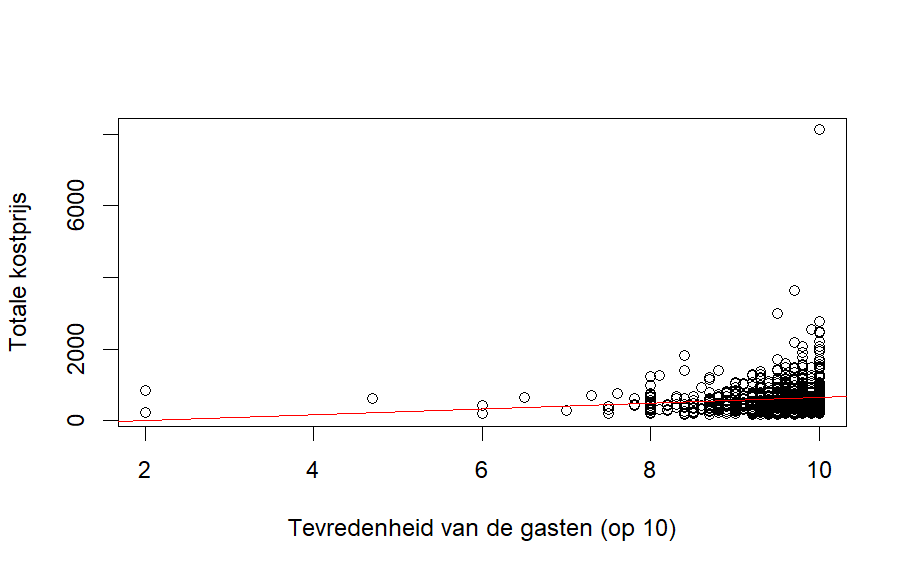
\includegraphics[width=0.49\linewidth]{Figuren/satis}
	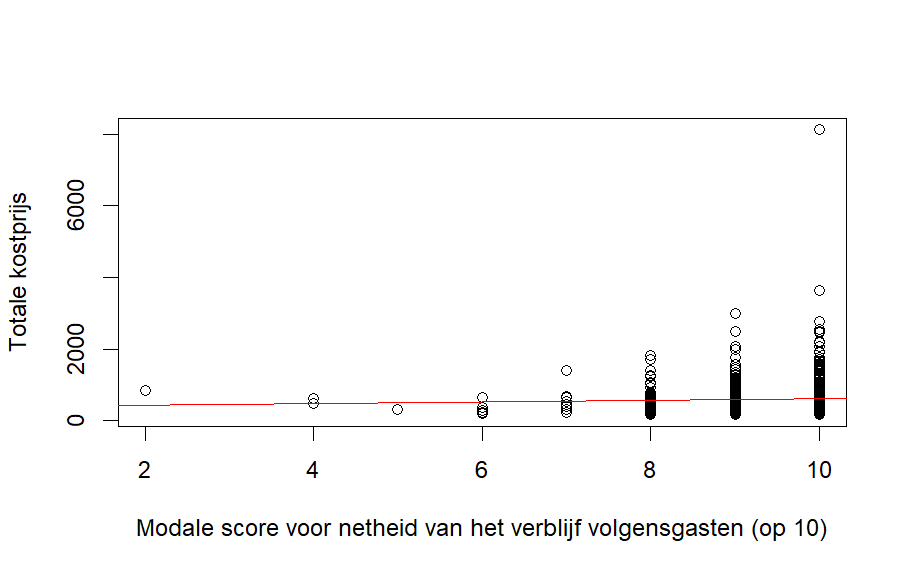
\includegraphics[width=0.49\linewidth]{Figuren/cleanliness}
	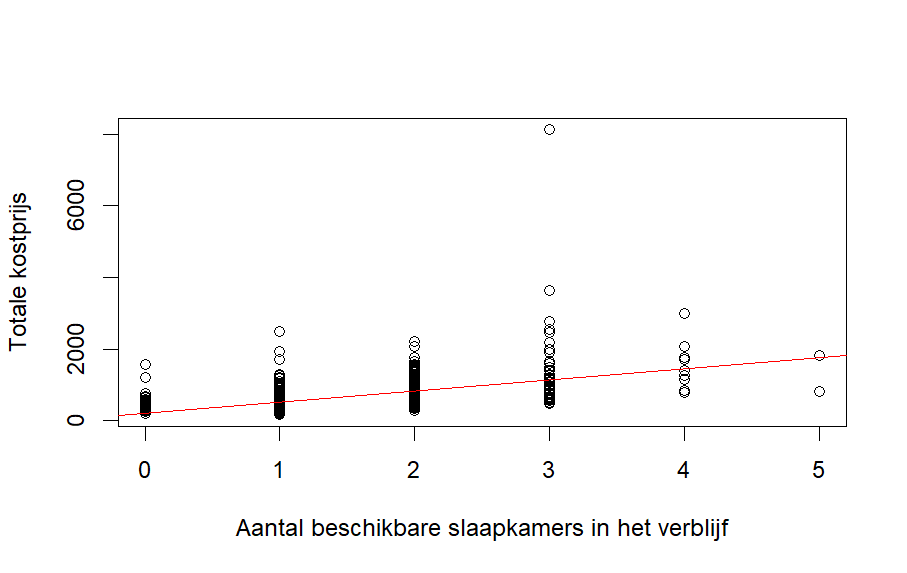
\includegraphics[width=0.49\linewidth]{Figuren/bedrooms}
	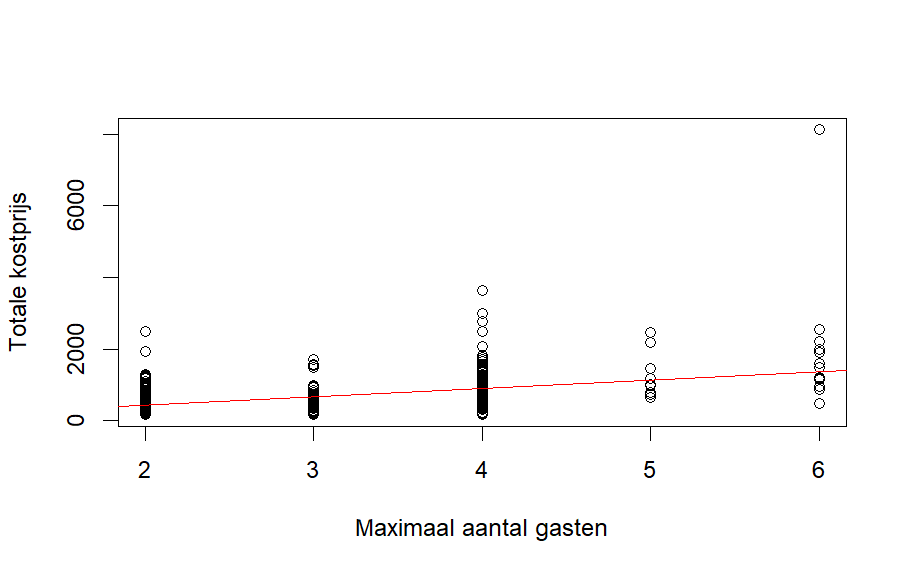
\includegraphics[width=0.49\linewidth]{Figuren/capacity}
	\caption{Scatterplots voor de totale prijs in functie van de andere veranderlijken}
	\label{fig:scatter}
\end{figure}
	\subsection{Verklaren van de kost}
	
	
	\section*{Besluit}
	%hebben we deze tabel ergens nodig?
	\begin{table}[h]
		\begin{tabular}{r*{2}{|r}}
			Veranderlijke & Uitkomst 1 & Uitkomst 2 \\ \hline
			Aantal &            &            \\ \hline
			Proportie &            &
		\end{tabular}
	\end{table}
\end{document} 